
I begin by validating the log-normality assumption at the tract level. Figure 1 examines the fit for median income, comparing observed values with those predicted under log-normality for each census tract, where observations are grouped into 25 equal-sized bins. The relationship is remarkably strong ($\beta$ = 0.98, $R^2$ = 0.98), with predicted values differing from observed ones by just 4.6\% on average. The near-unit slope coefficient and high R-squared indicate that log-normality captures the central tendency of the income distribution particularly well.

\begin{figure}[H]
\begin{center}
\captionsetup{justification=centering}
\caption{Validation of log-normality: median income}
\label{fig:median}
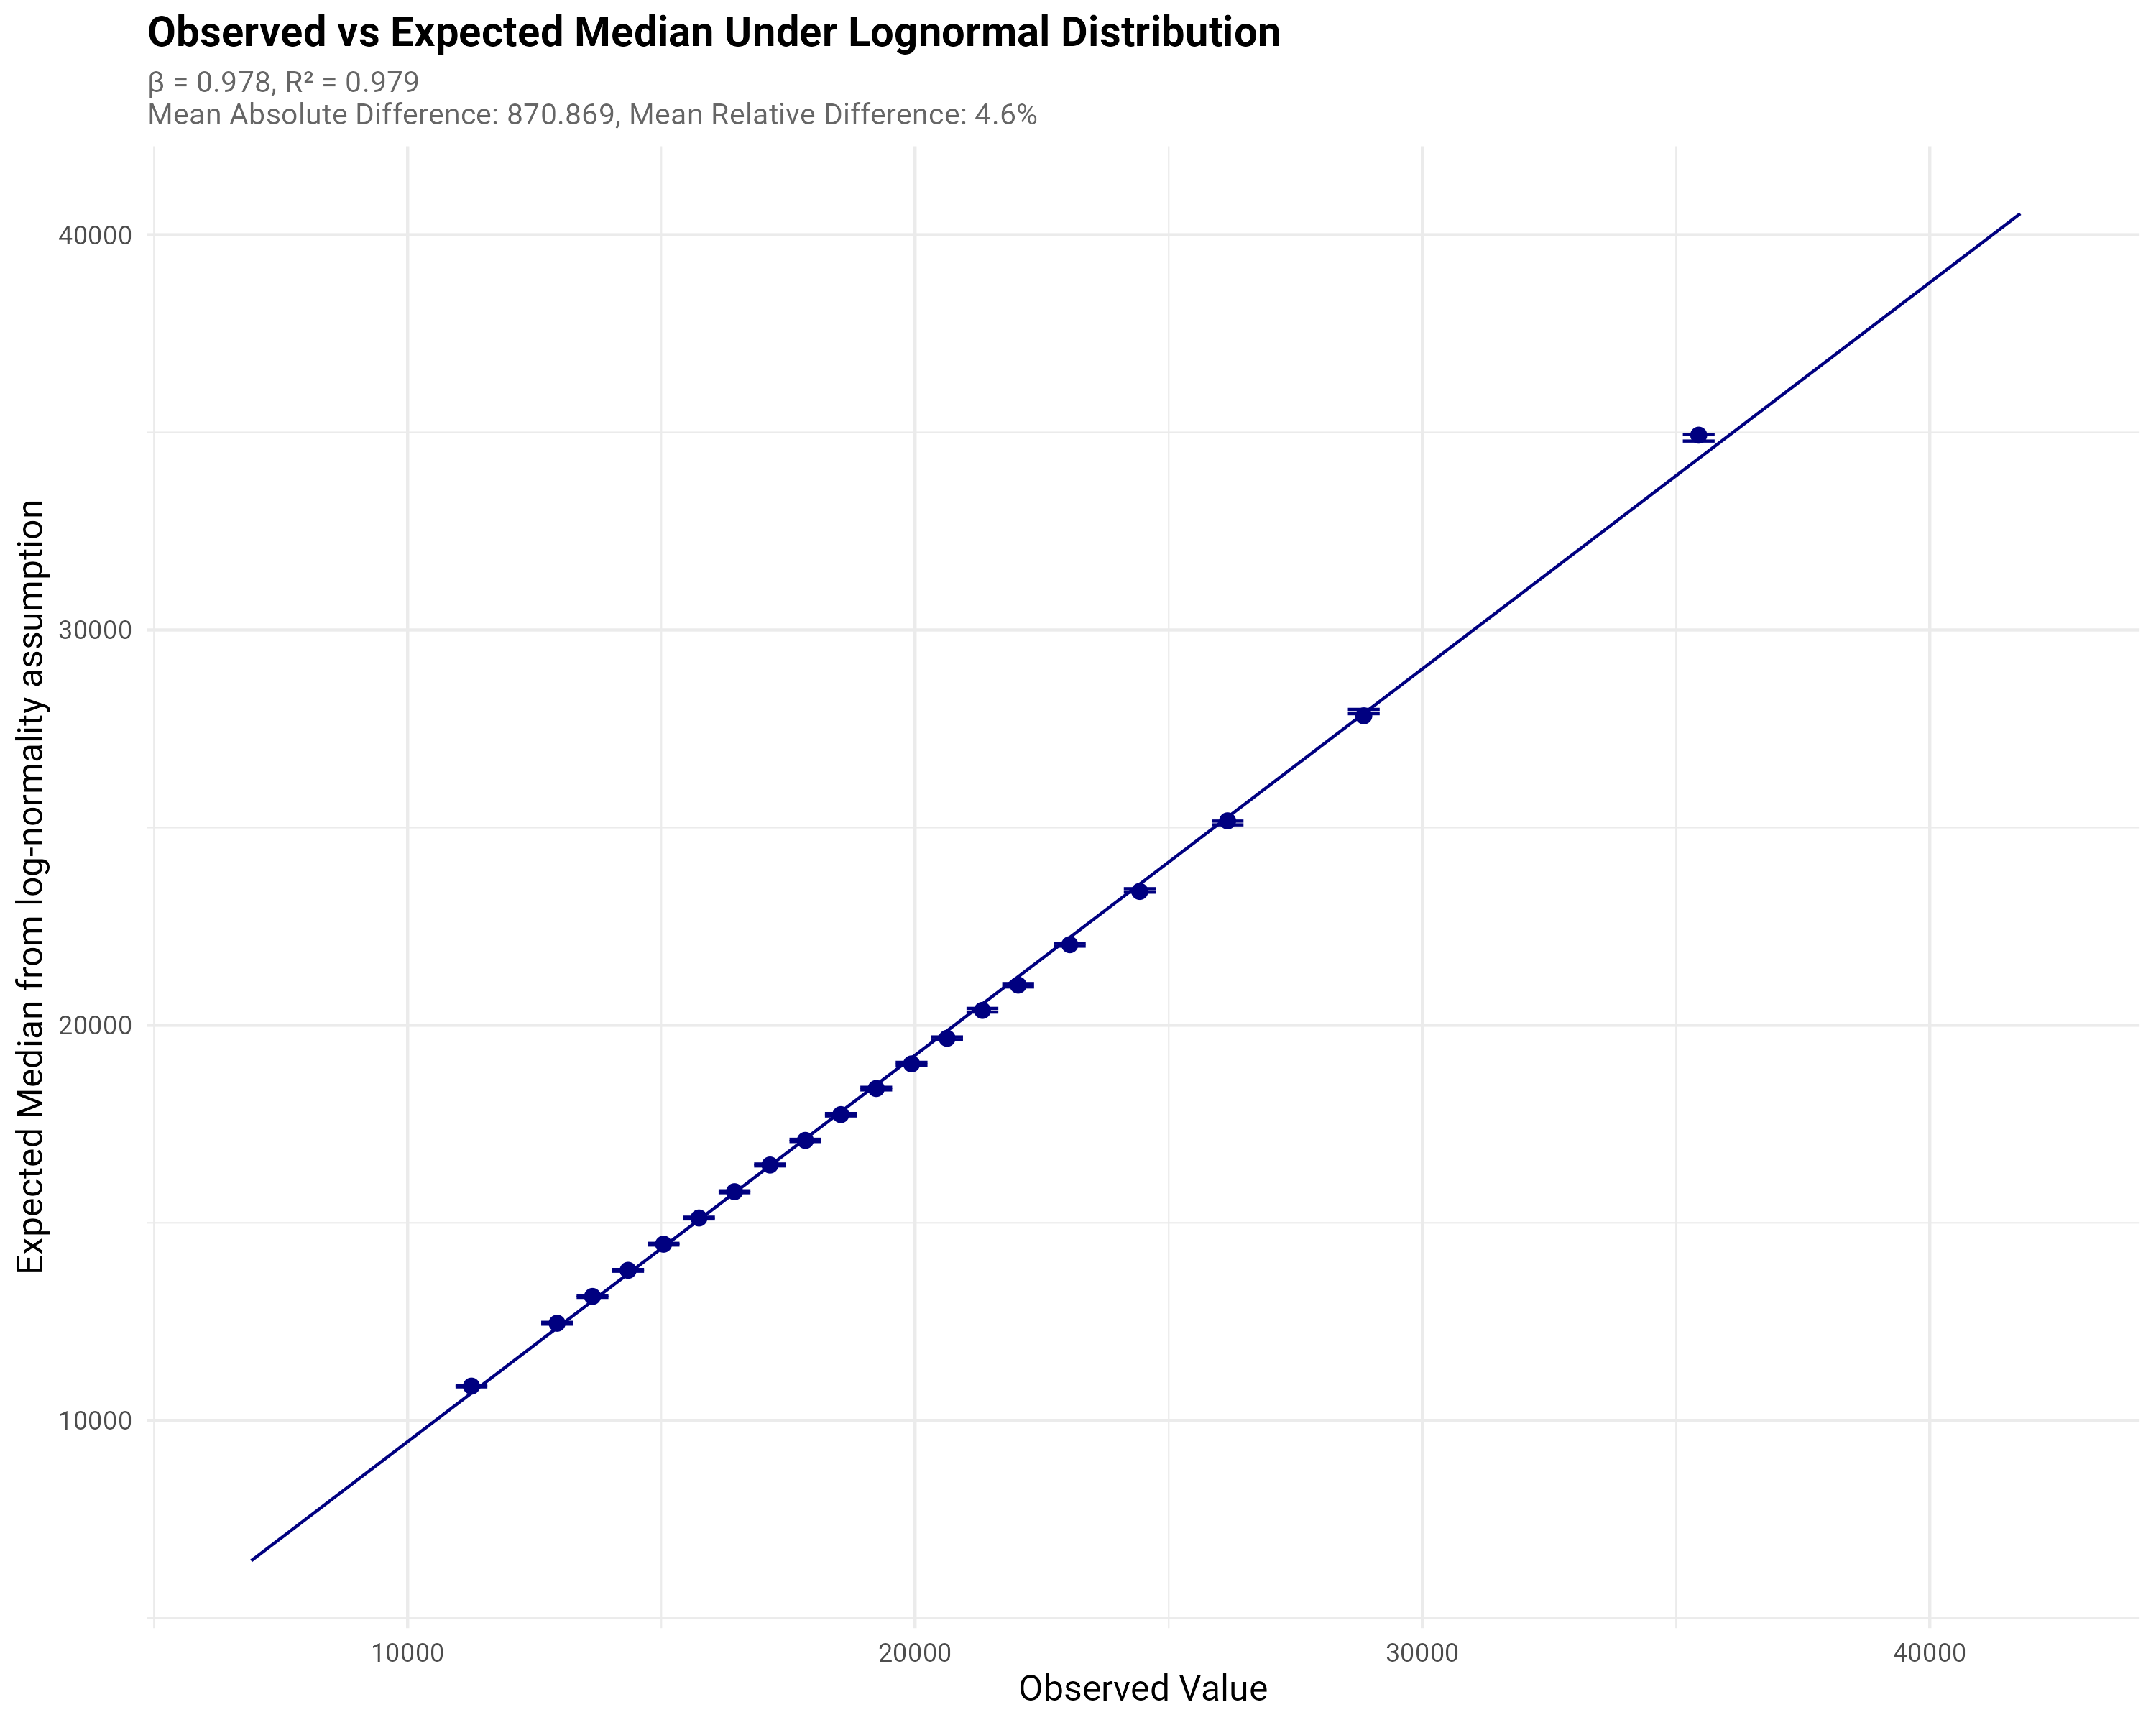
\includegraphics[width=0.8\textwidth]{output/binned_scatter_median.png}
\end{center}
\begin{fignotes2}
\textbf{Notes:} This figure shows a binned scatter plot comparing observed median income with predicted values under the log-normal assumption for each census tract. 
\end{fignotes2}
\end{figure}

Figure 2 shows the relationship for the P80/P20 ratio. The binned regression yields a slope coefficient of 0.75 ($R^2$ = 0.81), with predicted values deviating from observed ones by 5.0\% on average. Consistent with the fact that real income distributions tend to have heavier tails, the coefficient below unity suggests that the log-normal distribution slightly underestimates inequality.

\begin{figure}[H]
\begin{center}
\captionsetup{justification=centering}
\caption{Validation of log-normality: P80/P20 ratio}
\label{fig:p80p20}
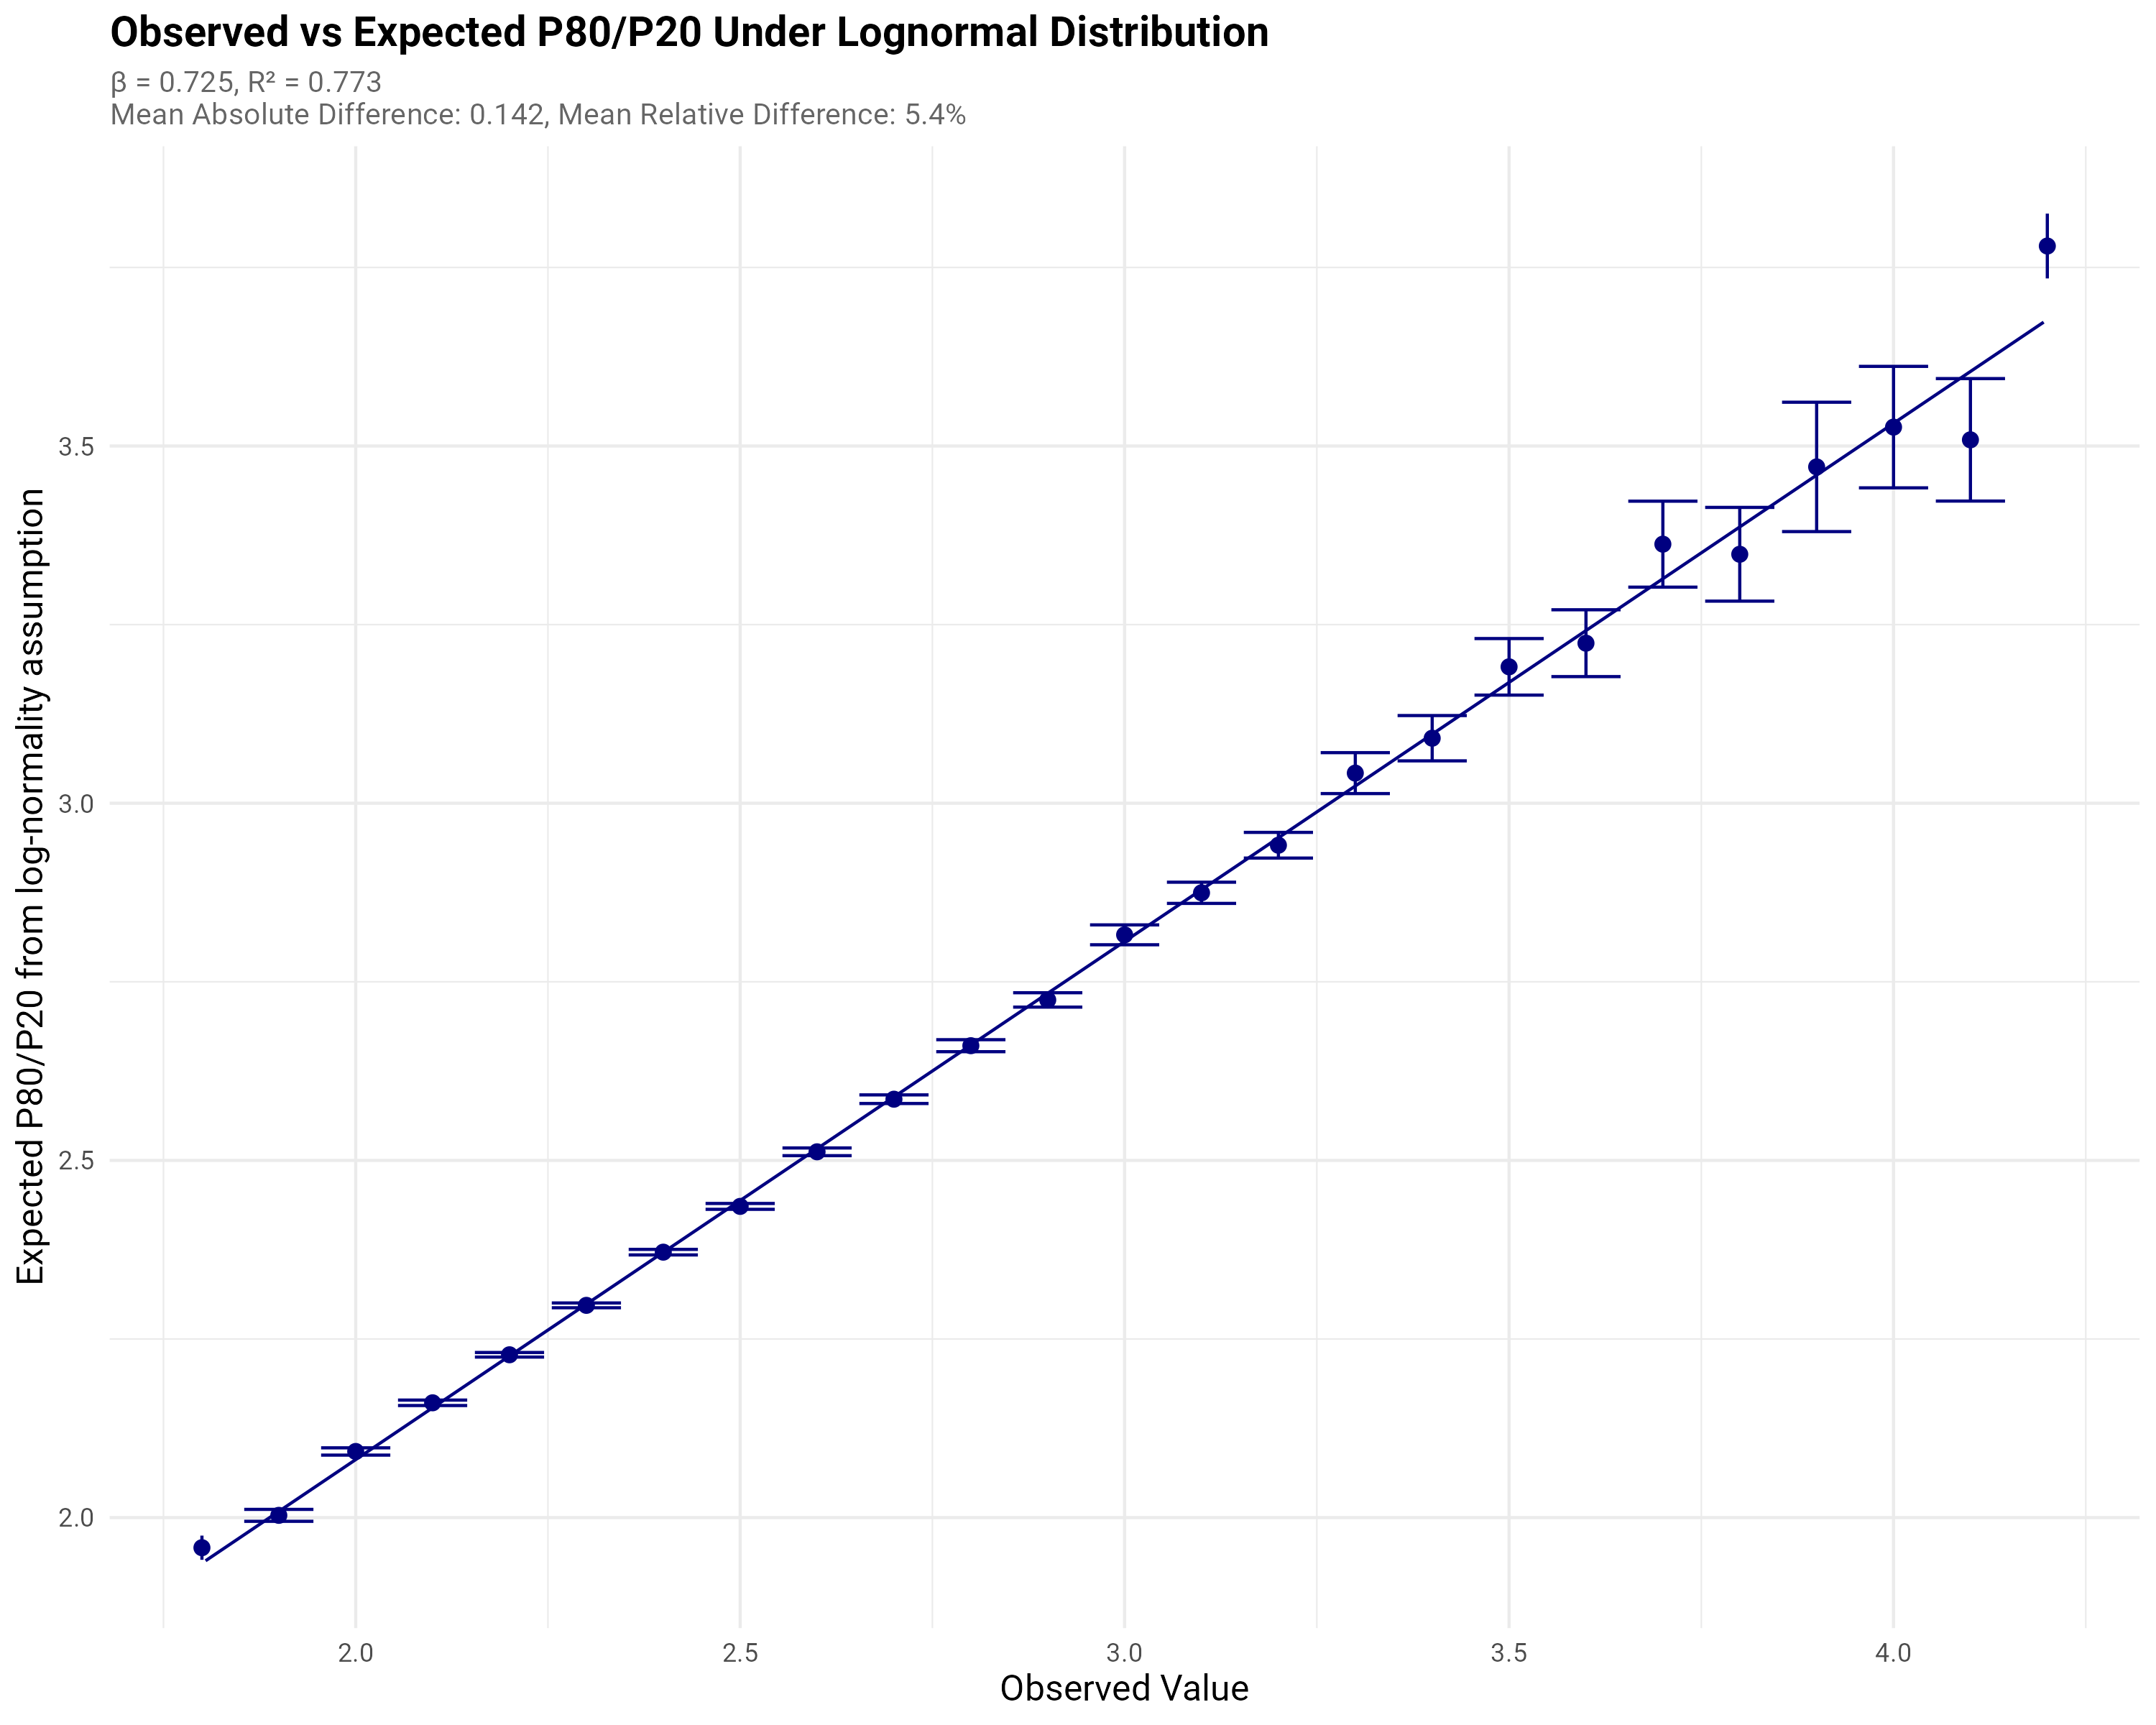
\includegraphics[width=0.8\textwidth]{output/binned_scatter_p80p20.png}
\end{center}
\begin{fignotes2}
\textbf{Notes:} This figure shows a binned scatter plot comparing observed P80/P20 ratios with predicted values under the log-normal assumption for each census tract.
\end{fignotes2}
\end{figure}

Next, I show how the mixture approach generates substantial differences between the distribution implied solely by tract means - where everyone within a tract is assumed to have the same income - and the estimated individual-level distribution. Figure \ref{fig:distributions} plots both distributions for net equivalised income in 2022. The tract-level distribution (in dark blue) exhibits higher kurtosis and is more concentrated around its mode of approximately €20,000, as it collapses all within-tract variation to a single point. In contrast, the estimated individual distribution (in red) shows greater dispersion and a lower mode, reflecting the within-tract inequality captured by the mixture of log-normal local distributions. The heavier left tail and more gradual right tail of the individual distribution suggest that a simple aggregation of tract means would vastly understate income inequality, particularly by failing to account for the substantial mass of low-income households and the long right tail of high earners.

\begin{figure}[H]
\begin{center}
\captionsetup{justification=centering}
\caption{Estimated income distribution vs. tract means}
\label{fig:distributions}
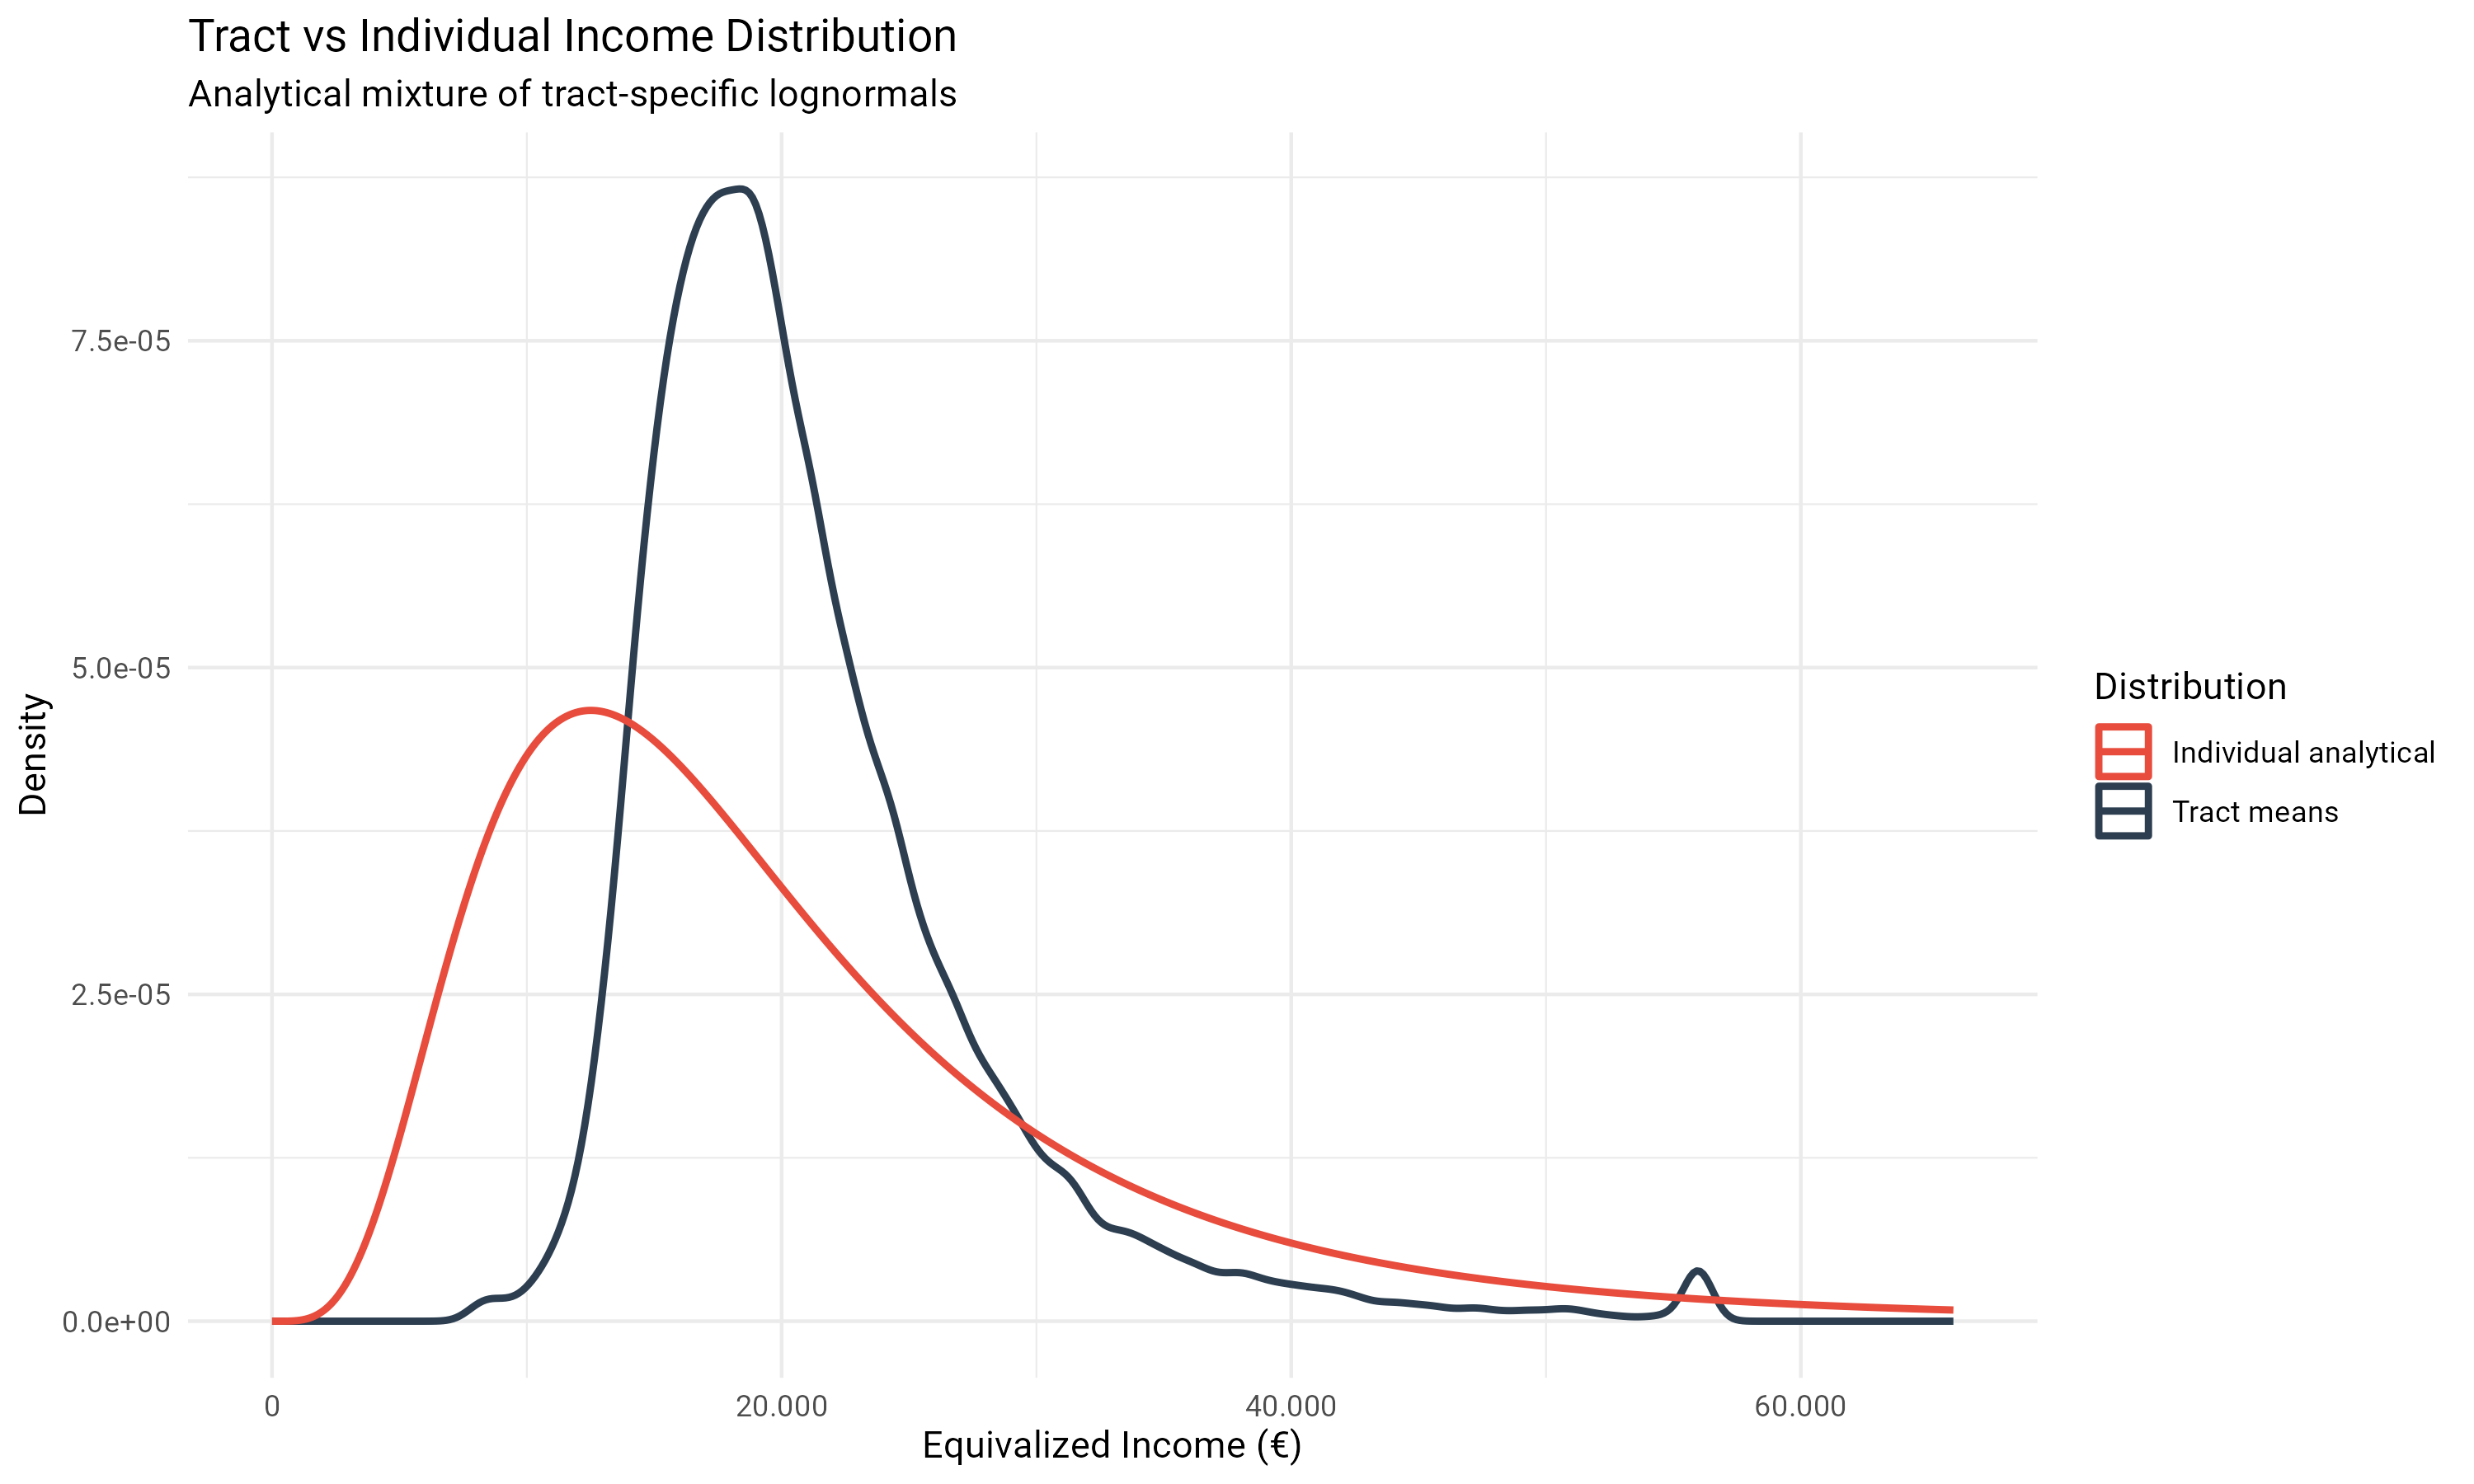
\includegraphics[width=0.8\textwidth]{output/tract_vs_individual_income_distribution.png}
\end{center}
\begin{fignotes2}
\textbf{Notes:} This figure shows two approaches to approximating the individual income distribution: using tract means (in dark blue), where everyone within a tract is assumed to have the same income, and using a mixture of log-normals (in red) that incorporates within-tract inequality. The tract means distribution is calculated as a population-weighted kernel density of tract means. The mixture distribution is constructed using tract-specific log-normal distributions, where the parameters of each component are derived from observed tract means and Gini coefficients, and mixture weights correspond to tract population shares.
\end{fignotes2}
\end{figure}


To better understand the spatial structure of income inequality in Spain, I decompose the total variance of log income into components corresponding to different geographic levels. This analysis helps validate the methodological approach by quantifying how much of the total income variation occurs within versus between different administrative units.
Specifically, I decompose the total variance of log income into four components:

Within-tract variation
Between-tract variation (within municipalities)
Between-municipality variation (within provinces)
Between-province variation

The within-tract component is calculated using the relationship between the Gini coefficient and the variance of log-normal distributions. The remaining components are computed using population-weighted variance decomposition methods.

\begin{figure}[H]
\begin{center}
\captionsetup{justification=centering}
\caption{Estimated income distribution vs. tract means}
\label{fig:distributions}
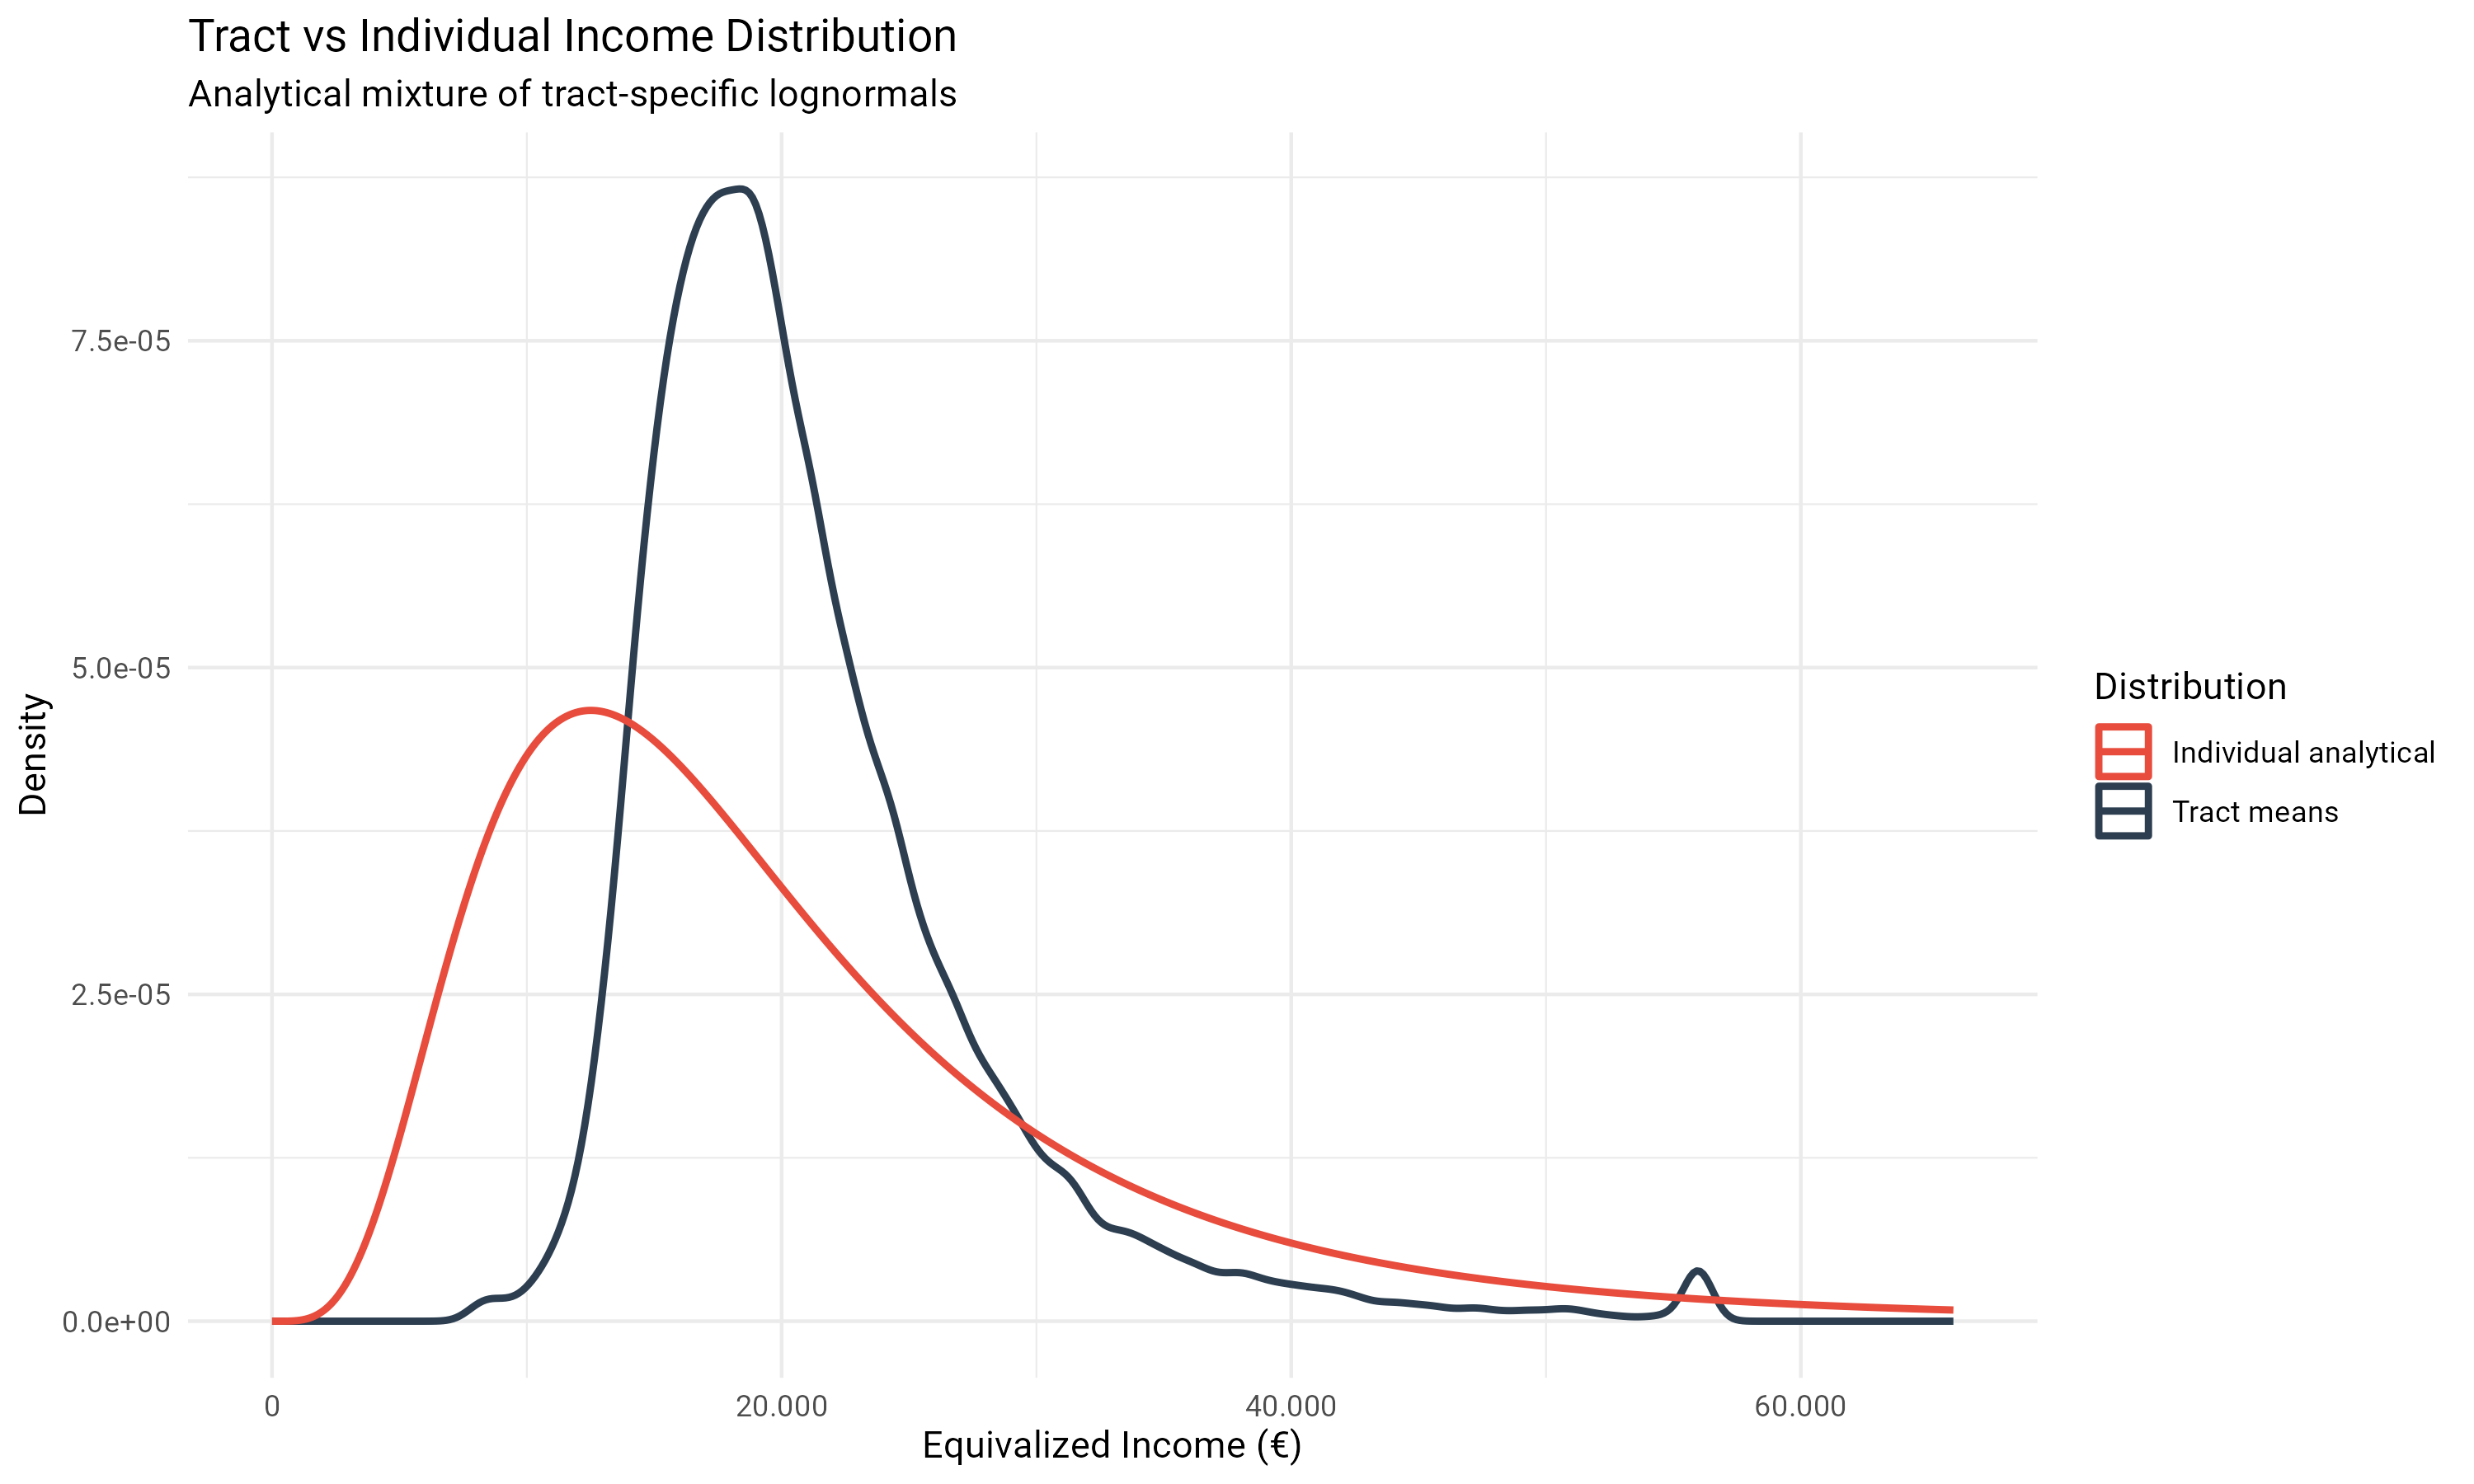
\includegraphics[width=0.8\textwidth]{output/tract_vs_individual_income_distribution.png}
\end{center}
\begin{fignotes2}
\textbf{Notes:} This figure shows two approaches to approximating the individual income distribution: using tract means (in dark blue), where everyone within a tract is assumed to have the same income, and using a mixture of log-normals (in red) that incorporates within-tract inequality. The tract means distribution is calculated as a population-weighted kernel density of tract means. The mixture distribution is constructed using tract-specific log-normal distributions, where the parameters of each component are derived from observed tract means and Gini coefficients, and mixture weights correspond to tract population shares.
\end{fignotes2}
\end{figure}